\chapter{Evaluation}
\label{chap:evaluation}
This chapter presents the evaluation results of the thesis. After some
remarks about the evaluation context in \refsec{sec:eval-context}, we
analyze the durations of different robot memory operations in
\refsec{sec:op-durations}. This includes comparing the durations for
different expressiveness levels and database sizes to find a
compromise between expressiveness and performance. Furthermore, we
analyze the overhead of database operations introduced by robot memory
features. In \refsec{sec:performance} we present the performance of
the system in the already introduced application scenarios. This
includes CPU and memory usage, network throughput, and statistics
about robot memory operations. Qualitatively, we evaluate how well the
features of the robot memory work, how it can support the development
of application scenarios, and where limitations are. Furthermore, we
present experiments regarding the compromise of expressiveness and
performance. \todo[inline]{review mentioning of all sections}

\section{Evaluation context}
\label{sec:eval-context}
The benchmarks presented in this chapter were performed on Fedora 23
systems with 16 GB RAM and an Intel Core i7-3770 with eight cores at
$3.4$~GHz. For local benchmarks everything, including Fawkes, MongoDB,
the Gazebo simulation and ROS, ran on a single system. For distributed
benchmarks, three identical systems were used. Each system hosted its
own Fawkes, ROS, and MongoDB processes and one system additionally,
hosts the Gazebo simulation.

Since the robot memory runs inside the Fawkes framework and thus
inside the Fawkes process, the performance of the robot memory can not
directly be measured separately and is influenced by Fawkes. The
influences are caused by other components, such as localization,
reasoning, and collision avoidance, and by the thread management of
Fawkes. To softly guarantee loop times for other threads, Fawkes
suspends threads with a too long loop iteration. When measuring
durations of robot memory operations, this can increase large
measurement values because if an operation takes longer than the
allowed loop iteration time, the time being suspended is added to the
measurement.

\section{Robot Memory Operations}
\label{sec:op-durations}
In this section, we analyze the run-time durations of robot memory
operations, such as insert, query, and update. We also analyze how
these change with computables and triggers. The goal is to find out
how fast the robot memory works. Besides the influence of the
implementation, the durations heavily depend on the underlying
complexity (e.g. of a query) and \emph{domain size}, which is the
amount of information stored in the robot memory. Here, we want to
find out how the durations scale with increasing domain size and
increasing complexity.

The structure of the data used for this evaluation is chosen in a way
that it is similar to information that is usually stored in a robot
memory and that it also simplifies the analysis. The used data mimics
a robot's knowledge about object and their positions to solve a tidy
up scenario. For each object, the robot memory contains a document
with the object's name, current position, and the storage position it
belongs to. Names are unique and storage positions are randomly chosen
out of $1000$ possibilities. Objects are currently placed at their
storage position with probability $0.01$ and random otherwise. The
object's name is string to enforce string comparisons, which are
expected to be often needed in a real scenario. For evaluation
reasons, we do not index the collection by the s name right now
because this heavily impacts the duration. An evaluation plugin in
Fawkes generates the data and calls random operations. To analyze how
the durations scale with the domain size, the plugin calls the
operations repeatedly after increasing the domain size from $0$ to
$100000$ documents by steps of $1000$ documents.

The analysis is separated into the main classes of operations, namely
insertions in \refsec{sec:insertions}, queries in
\refsec{sec:queries}, and updates in \refsec{sec:updates}. Because
deletions behave very similar to updates, both search for documents
and work with them, they are also covered in the section about
updates. \refsec{sec:eval-computables} covers and explains the impact
of computables on query durations and \refsec{sec:eval-trigger} deals
with the impact of event triggers. Operations that are performed
rarely are not analyzed. For example dropping or restoring a collection and
registration of triggers and computables are only performed once
during initialization.  In the course of implementing and evaluating
the application scenarios, their durations were not noticeable compared
to the initialization time of the whole robot software.

\subsection{Insertions}
\label{sec:insertions}
\begin{figure}
  \centering
  \begin{subfigure}[b]{0.49\textwidth}
    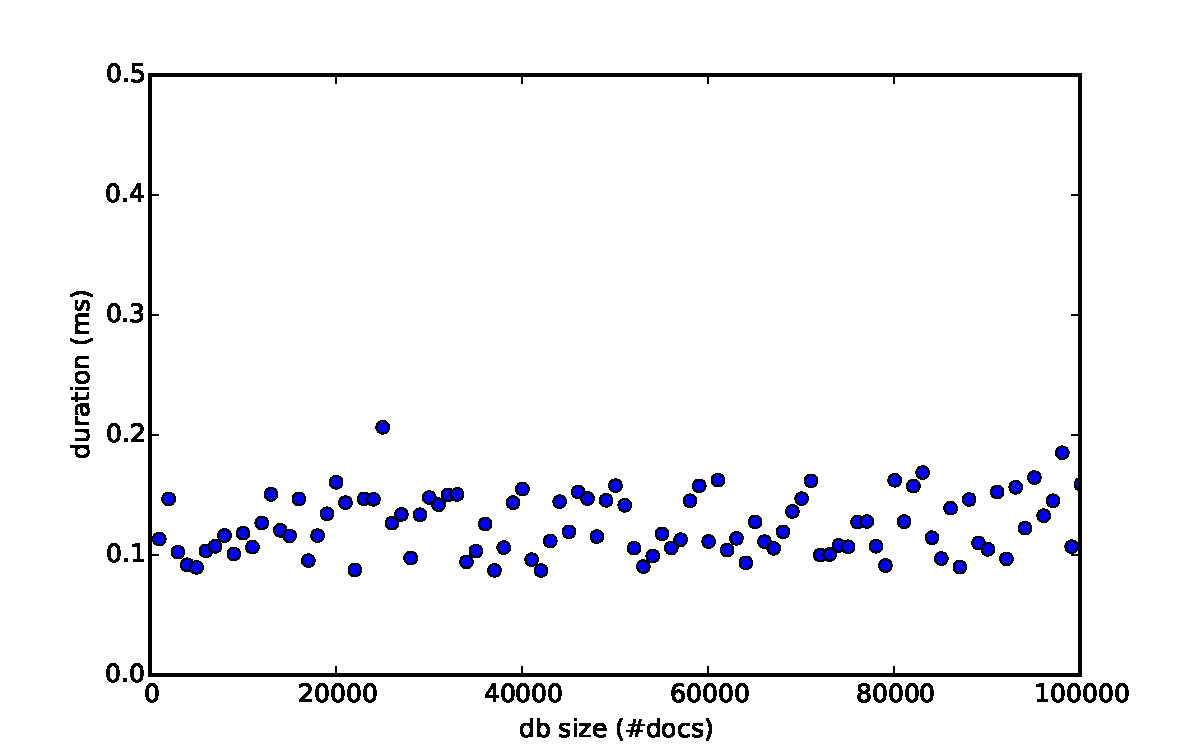
\includegraphics[width=\textwidth]{plots/insert-durations}
    \caption{Insertions}
    \label{fig:insert-durations}
  \end{subfigure}
  \begin{subfigure}[b]{0.49\textwidth}
    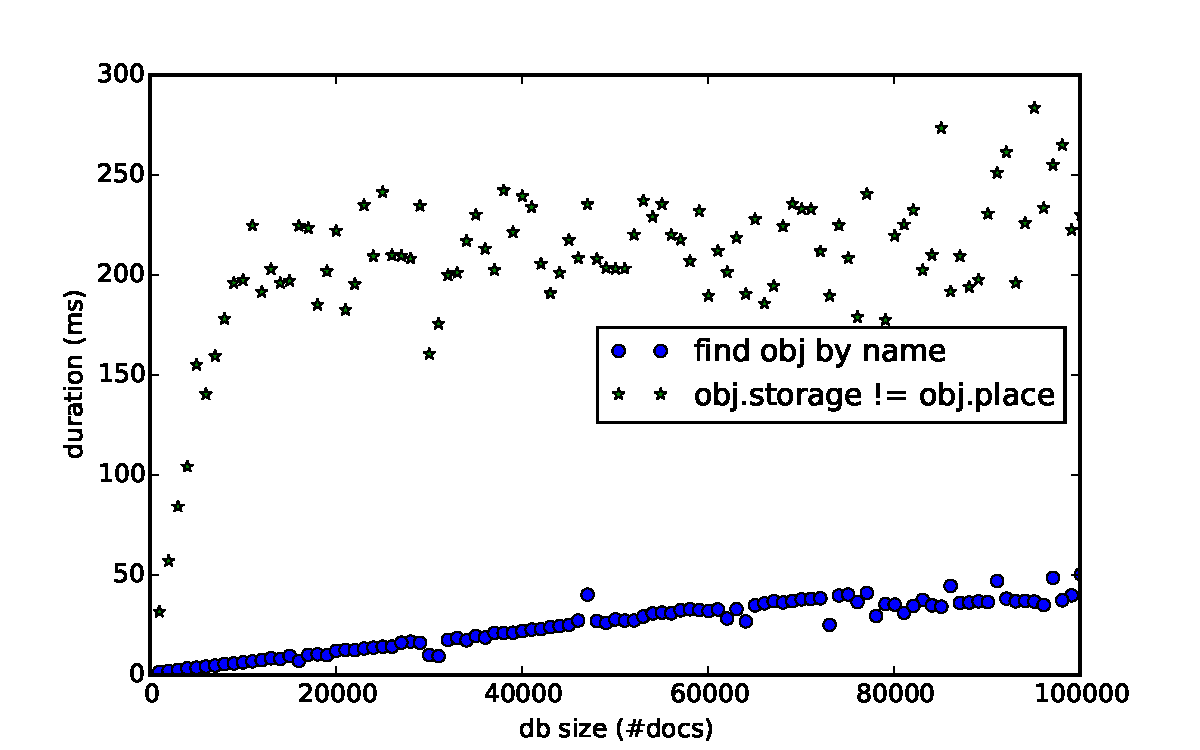
\includegraphics[width=\textwidth]{plots/query-durations}
    \caption{Queries}
    \label{fig:query-durations}
  \end{subfigure}
  \caption[Duration of robot memory operations with increasing domain size]{Duration of robot memory operations with increasing domain size}
  \label{fig:eval-durations-1}
\end{figure}
The insertion of a new document into the robot memory is overall the
fastest operation compared to queries and
updates. \reffig{fig:insert-durations} shows the distribution of
insert durations with increasing domain size. It is noticeable that the
duration does not depend on the domain size and thus has run-time
complexity of $O(1)$. The insertion time is small with an average of
$0.125ms$. However, there are single outliers not present in
\reffig{fig:insert-durations}. These outliers occur periodically, when
MongoDB flushes database changes from the RAM to the hard drive. We
could reduce frequency of these outliers to one in $60s$, which is the
default flushing frequency of MongoDB. To reach this, we had to
disable the forward logging of MongoDB, called Journaling. In this
evaluation scenario, the outliers took about $0.3s$ because of the
large amount of written documents and the threading in Fawkes.  The
overhead of the robot memory compared to the duration of the raw
MongoDB operation has an average of $0.006ms$, which is about $5.5\%$.
The overhead is caused by verifying the collection name, deciding if
the local or distributed database is used, adding meta-data, and
mutual exclusion of database usage. The robot memory overhead measured
here does not include checking if triggers were activated by inserting
the document. This is caused by the asynchronous and separate checking by
the trigger manager. The size and the complexity of inserted
documents did not make a noticeable difference.\todo{need to add
  numbers?}

\subsection{Queries}
\label{sec:queries}
Queries are more complex operations than insertions and also take more
time. \reffig{fig:query-durations} shows that query durations heavily
depends on many factors, such as domain-size and query complexity. The
query durations, when searching for an object by it's unique name,
linearly depend on the domain size. The other plot shows the query
durations for finding objects that are not at their storage location
and thus would have to be tidied up. The query is more complex
because it contains a comparison between two values that is formulated
in JavaScript. From $0$ to about $10000$ documents, also a linear
increase can be seen. With more documents the average duration does
not increase, because of a query evaluation trick of MongoDB. MongoDB
lazily evaluates queries and returns a cursor to the first batch of
documents that match the query. While the user iteratively fetches
documents from the cursor, MongoDB continues the query evaluation if
the batch was emptied. For the 'find object name' query, the whole
database was searched because the unique object could not fill the
batch. However it is possible to request a smaller batch (e.g. only
one) document for faster computation.  \todo[inline]{comparison with
  indexing} The overhead of the robot memory query operation does not
depend on the domain size and has an average duration of $0.6ms$. The
largest part of that overhead is caused by the computable manager,
even if in this scenario no computables are registered. The computable
manager performs a single insert and remove on a separate collection
to prepare checking if the query matches a computable and to clean up
afterwards. Because of this insertion, the duration spikes observed
for insertions can also occur for queries.  \todo[inline]{more
  different query complexities?}  As \reffig{fig:query-durations}
shows, the query duration heavily depends on the complexity of the
query. Especially the expressive JavaScript functions are expensive
compared to the MongoDB internal query language without JavaScript. By
formulating queries smartly, complex questions can often be
efficiently in practice. For example checking whether the dishwasher
is full sounds like a question that is computationally costly because
it requires JavaScript function. But it can be formulated efficiently
by first filtering only the objects in the dishwasher with a fast
JavaScript-free query and then summing up the objects volume to check
if it exceeds a given threshold. This way the costly sum computation,
which can be done by aggregation or JavaScript, only needs to be
computed for the few objects in the dishwasher.
  \todo[inline]{concrete example for query formulation?}
  \todo[inline]{aggregation/map-reduce graph?}

\subsection{Updates and Deletions}
\label{sec:updates}
\begin{figure}
  \centering
  \begin{subfigure}[b]{0.49\textwidth}
    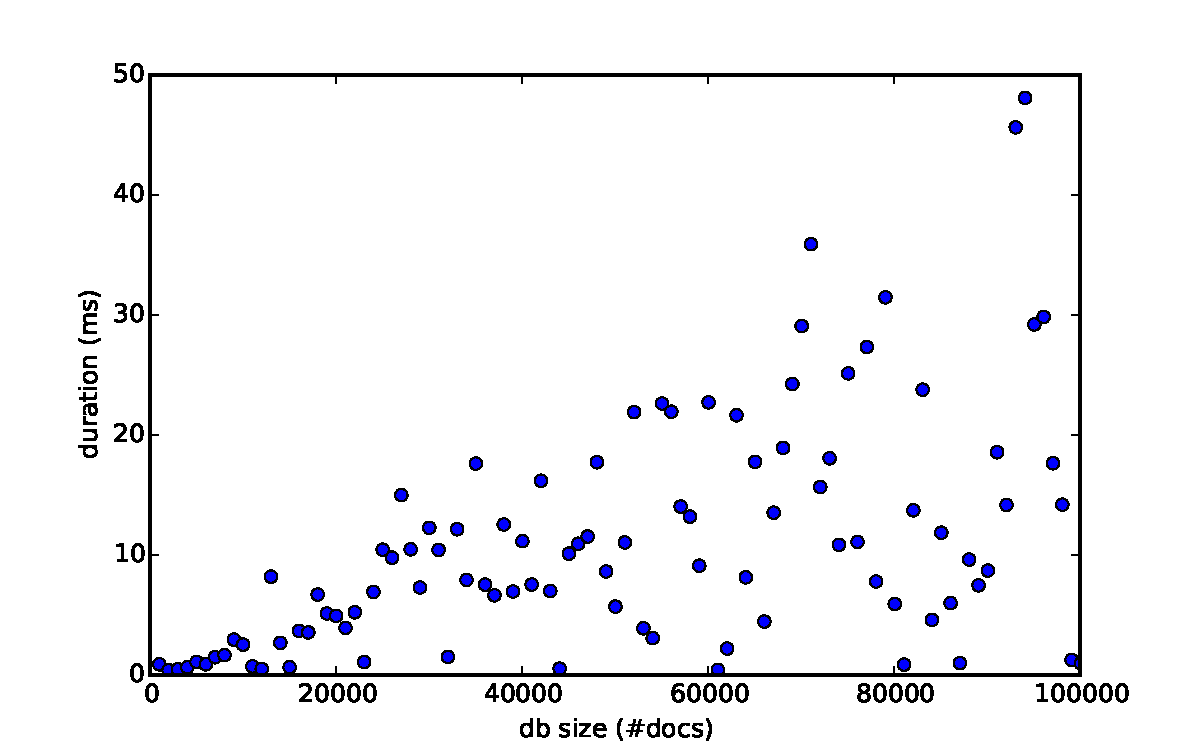
\includegraphics[width=\textwidth]{plots/update-durations}
    \caption{Updates}
    \label{fig:update-durations}
  \end{subfigure}
  \begin{subfigure}[b]{0.49\textwidth}
    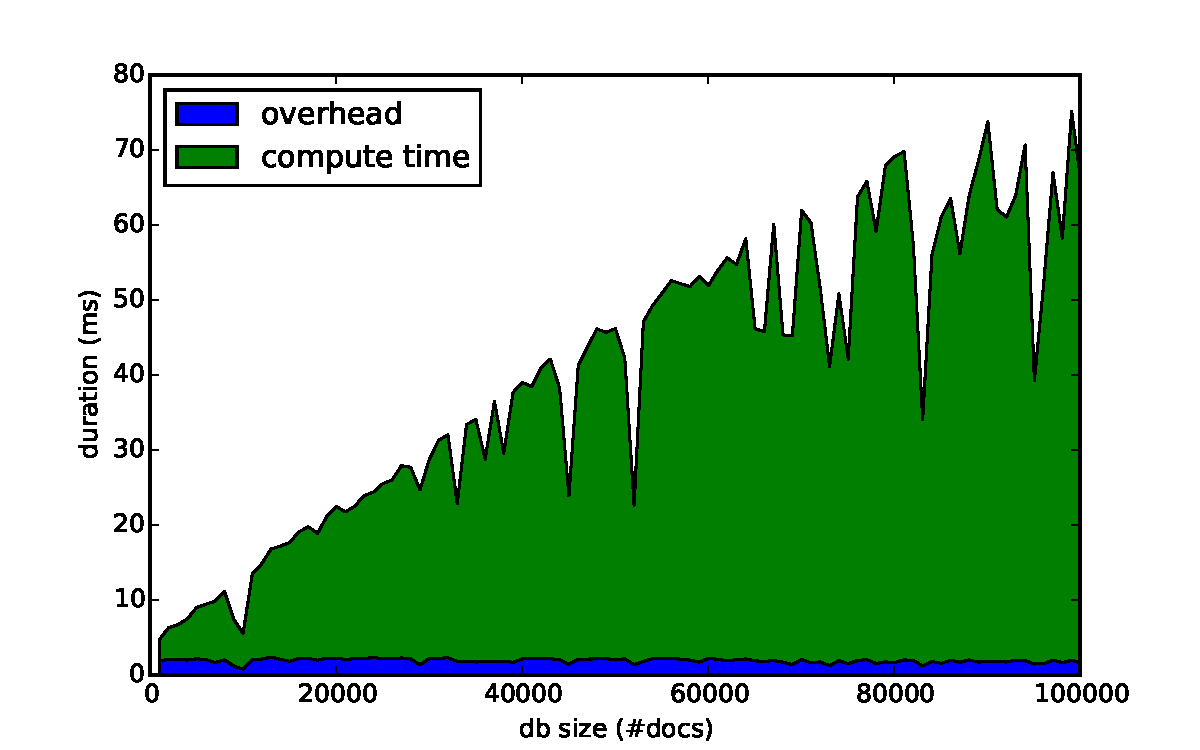
\includegraphics[width=\textwidth]{plots/computable-durations}
    \caption{Computables}
    \label{fig:computable-durations}
  \end{subfigure}
  \caption[Duration of robot memory operations with increasing domain size]{Duration of robot memory operations with increasing domain size}
  \label{fig:eval-durations-2}
\end{figure}
Updates consist of a query defining what should be updated and some
key-value pairs, which should be changed. Thus the duration of an
update should be similar to an update plus an
insertion. \reffig{fig:update-durations} shows the duration of
position updates of objects with a random name. Because the used
update operation only updates a single document, the durations are
roughly uniformly distributed with an upper bound matching the
duration of 'find object' queries in
\reffig{fig:query-durations}. Thus the duration of update operations
also scale linearly with the domain size. Duration of queries
searching for only one document also behave as in
\reffig{fig:update-durations}.  Because delete operations also consist
of a query and a fast change operation, they behave similar to
updates. The difference is that by default deletions are executed on
all documents and updates only on a single one. For both deletions and
updates the overhead does not depend on the database size. Both
updates and deletions have an average overhead duration below
$0.02ms$. In contrast to to query operations, the computable manager
is not involved, because computed documents should not be updated and
they do not need to be removed manually.

\subsection{Computables}
\label{sec:eval-computables}
Computables generate new information when it is demanded by a
query. Thus each new query is checked by the computable manager as
explained in \refsec{sec:queries}. \reffig{fig:computable-durations}
shows the time needed for checking if a query demands a computable and
for computing the results. The computable used in
\reffig{fig:computable-durations} calculates the distance of the robot
to the closest object in the database and yields the object's name,
position, and distance. The measurement does not include the query
duration to of finding the computed document. The computation time of
the computable itself scales linear with the domain size because each
object's distance needs to be checked. The time of the overhead does
not depend on the domain size. The overhead includes inserting the
original query in MongoDB, evaluating the demand query for each
registered computable to check if the original query demands the
computable, and a clean up operation. Furthermore, the results of the
computable need to be inserted into the robot memory. Asynchronously
in the main loop of the robot memory, computed documents are removed
again. Thus the time needed for computables depends on the amount of
registered computables, the amount of computed documents, and mainly
the computation time needed for each matching computable itself. This
computation time can get large if the computable solves problems with
higher complexity. For example a computable that finds the pair of
objects with the smallest distance to each other would scale
quadratically with the domain size. To avoid repeated computation of
the same data, we implemented caching for computables. As long as
specified by the caching time, the computation step is skipped if the
new query is identical to the query that demanded the computation
before. The remaining overhead of the computable manager is the same.

\subsection{Trigger}
\label{sec:eval-trigger}
Triggers notify an application when something in the database changes
as specified in the trigger query. For this benchmark, we registered a
trigger on new objects in a certain location (e.g. in the laundry
box). If trigger events happened, is checked each loop iteration of
the robot memory by the trigger manager. Because trigger queries,
which check for these events, are only executed on the Oplog and not
on the whole database, the time needed to check trigger depends on the
amount of registered trigger and the amount of database changes
(insertions, updates, and deletions). The current domain size has no
influence. During the insertion of the $100000$ objects, the trigger
manager checked for trigger events $2249$ times with an average
duration of $0.27ms$. That makes $0.006ms$ per insertion. This
duration also depends heavily on the formulation of the trigger query
(e.g. in the case of JavaScript usage). These measurements do not
include the computation time needed by the callback function of the
trigger. Because the callback function is executed directly, it's
computation time influences the loop time of the robot memory and can
in the worst case block it.

\section{Performance in evaluation scenarios}
To evaluate the performance of the robot memory, we performed
benchmark in multiple application scenarios. The measurements during
the experiments were stored and plotted using benchmarks were made
with the Round Robin Database Tool (RRD) as in~\cite{RoboDB}. The
first scenario is a simulated RoboCup Logistics League game, in which
the synchronization of the worldmodel between the robots was
implemented with the robot memory.
\label{sec:performance}
\begin{figure}
  \centering
  \begin{subfigure}[b]{1\textwidth}
    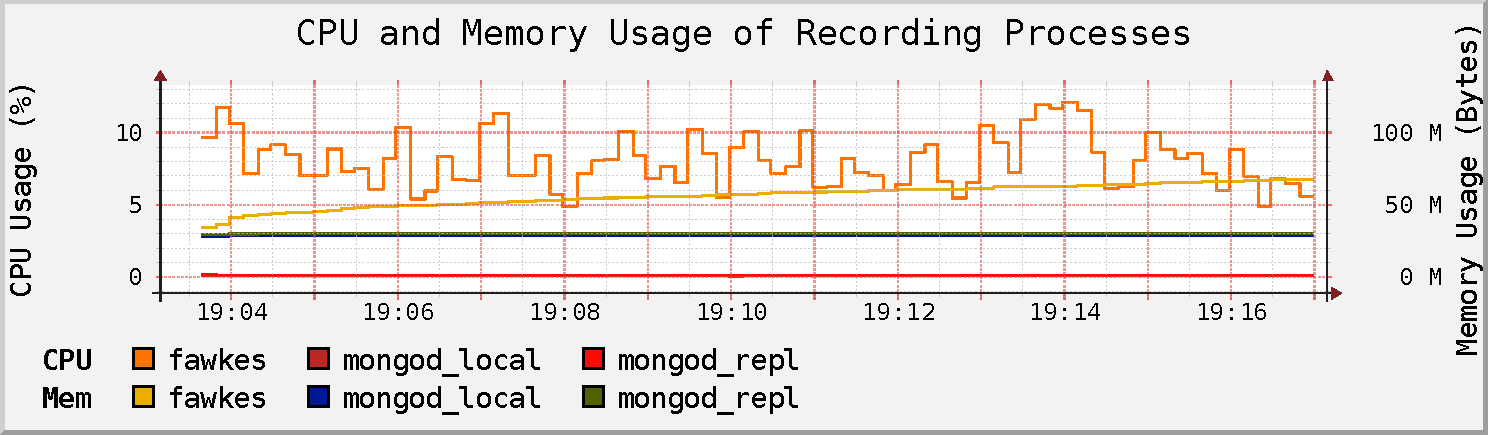
\includegraphics[width=\textwidth]{plots/rcll-local/cpu-mem}
    \label{fig:rcll-cpu-mem}
  \end{subfigure}
  \begin{subfigure}[b]{1\textwidth}
    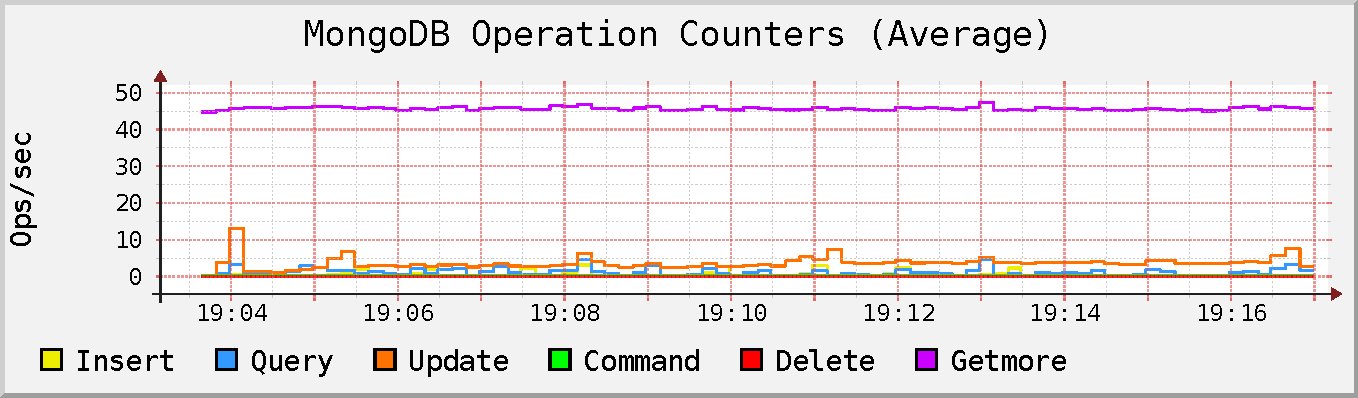
\includegraphics[width=\textwidth]{plots/rcll-local/operations}
    \label{fig:rcll-ops}
  \end{subfigure}
  \caption[Benchmark during a locally simulated RCLL game]{Benchmark during a locally simulated RCLL game}
  \label{fig:rcll-benchmark}
\end{figure}
\reffig{fig:rcll-benchmark} show the CPU and memory usage, as well as
the operations performed by MongoDB. For clarity only the CPU and
memory usage of one Fawkes instance of the three robots is
plotted. Both MongoDB processes, one for the robot local robot memory
and one for the distributed worldmodel, have a CPU usage below $1\%$
and a memory usage below $40MB$. This is not surprising because the
robot's world model that needs to be synchronized in the RCLL only has
a size of $60$ to $100$ documents with an average object size of $390$
bytes. It only grows slowly because most of the documents are updated
and there are few new documents for incoming orders and and work-pieces
in production. This is also shown by the MongoDB operation count shown
in \reffig{fig:rcll-benchmark}, which matches the operation count of
the robot memory well. The values include the database operations of
all three robots. \reffig{fig:rcll-benchmark} shows that the mostly
used operation is the \emph{Getmore} operation, which checks for an
existing query cursor if there are more matching documents than in the
previous batch. This is caused by the computable manager because it
periodically checks the Oplog for new changes that have to be reported
to the CLIPS agent. Since the robot memory runs inside the Fawkes
process, it's CPU and memory usage is included in the values of Fawkes
in \reffig{fig:rcll-benchmark}. The growing memory usage of Fawkes is
also present in benchmarks of the RCLL simulation without the robot
memory and the CPU curve looks similar. Thus the robot memory plugin
has no large impact on the performance in this scenario. \todo{mention
amcl,colli, reasoning because they cause most CPU usage of Fawkes?}
\todo[inline]{Also show RCLL graph without robot memory? (looks
  boringly similar, but might be satisfying for the reader to verify)}
\todo[inline]{Comparison to Synchronization with protobuf messages
  (re-syncing feature of MongoDB, not always sending whole world
  model...)}
The size of the database on the hard-drive is about $1097MB$ for the
distributed part and $1060MB$ for each local one. The size does not
change noticeably over time. $1GB$ of each database is occupied by the
Oplog, which has a constant size because it is a capped collection.


local/distributed

ops:
Getmore:trigger checks, otherwise mostly updates of the worldmodel
insertion of initial worldmodel skipped

data scenario: arm

\section{Qualitative Evaluation}
\todo[inline]{qualtitative eval: refer to goals from approach as structure}
\todo[inline]{refine qualitative structure}
\todo[inline]{for eval of Special Views for Different Components}
%% example queries/ key-translations and computable for hybrid transformations
\todo[inline]{for eval of computation on demand:}
%% For example it would be possible to add
%% a commonsense reasoner similar to KnowRob or ORO providing computables
%% to the robot memory. Queries for this commonsense knowledge would then
%% be forwarded to the commonsense reasoner and be solved by relating
%% knowledge in the memory to an ontology.

\todo[inline]{eval shared memory multi-robot system}
%% If the distribution of the
%% knowledge would not be implemented in the robot memory it would have
%% to be implemented separately. 
\todo[inline]{eval human interface + vis}
%% robomongo, robot memory operations over webview messages, visualization as in evaluation plots 
\todo[inline]{flaw: trigger on computables not possible without invoking computable by some query}
\todo[inline]{flaw: debugging communication (with computables) difficult becasue of flexibility (no error, but just no documents returned on query)}
\todo[inline]{Difference simulation-real world (almost same for robot memory, no possibility to test because of missing field, but distribution and full game already tested)}